
\subsection{PAH band ratios}
\label{sect:pah_ratios}

Both the 6.2 and 7.7~$\mu$m features are thought to be coming from ionized PAHs and the 11.3~$\mu$m feature from neutral PAHs. Therefore we expect to see a correlation between the intensities of 6.2 and 7.7~$\mu$m PAH features normalized by the 11.3~$\mu$m feature.  Figure \ref{PAHlines}  compares the PAH flux ratios of 7.7/11.3  and 6.2/11.3 features. The figure shows a good correlation between these two PAH line ratios, consistent with that of the SINGS sample shown by \citet{Smith:2007lr}.
A similar correlation was also reported by  \citet{Galliano2008} for a sample of galaxies and a handful of extended H{\sc ii} regions
and by \citet{Vermeij2002} for Galactic and Magellanic Cloud H{\sc ii}regions. This provides evidence that the PAH emission from M31 is not unusual. 


\begin{figure}
\centering
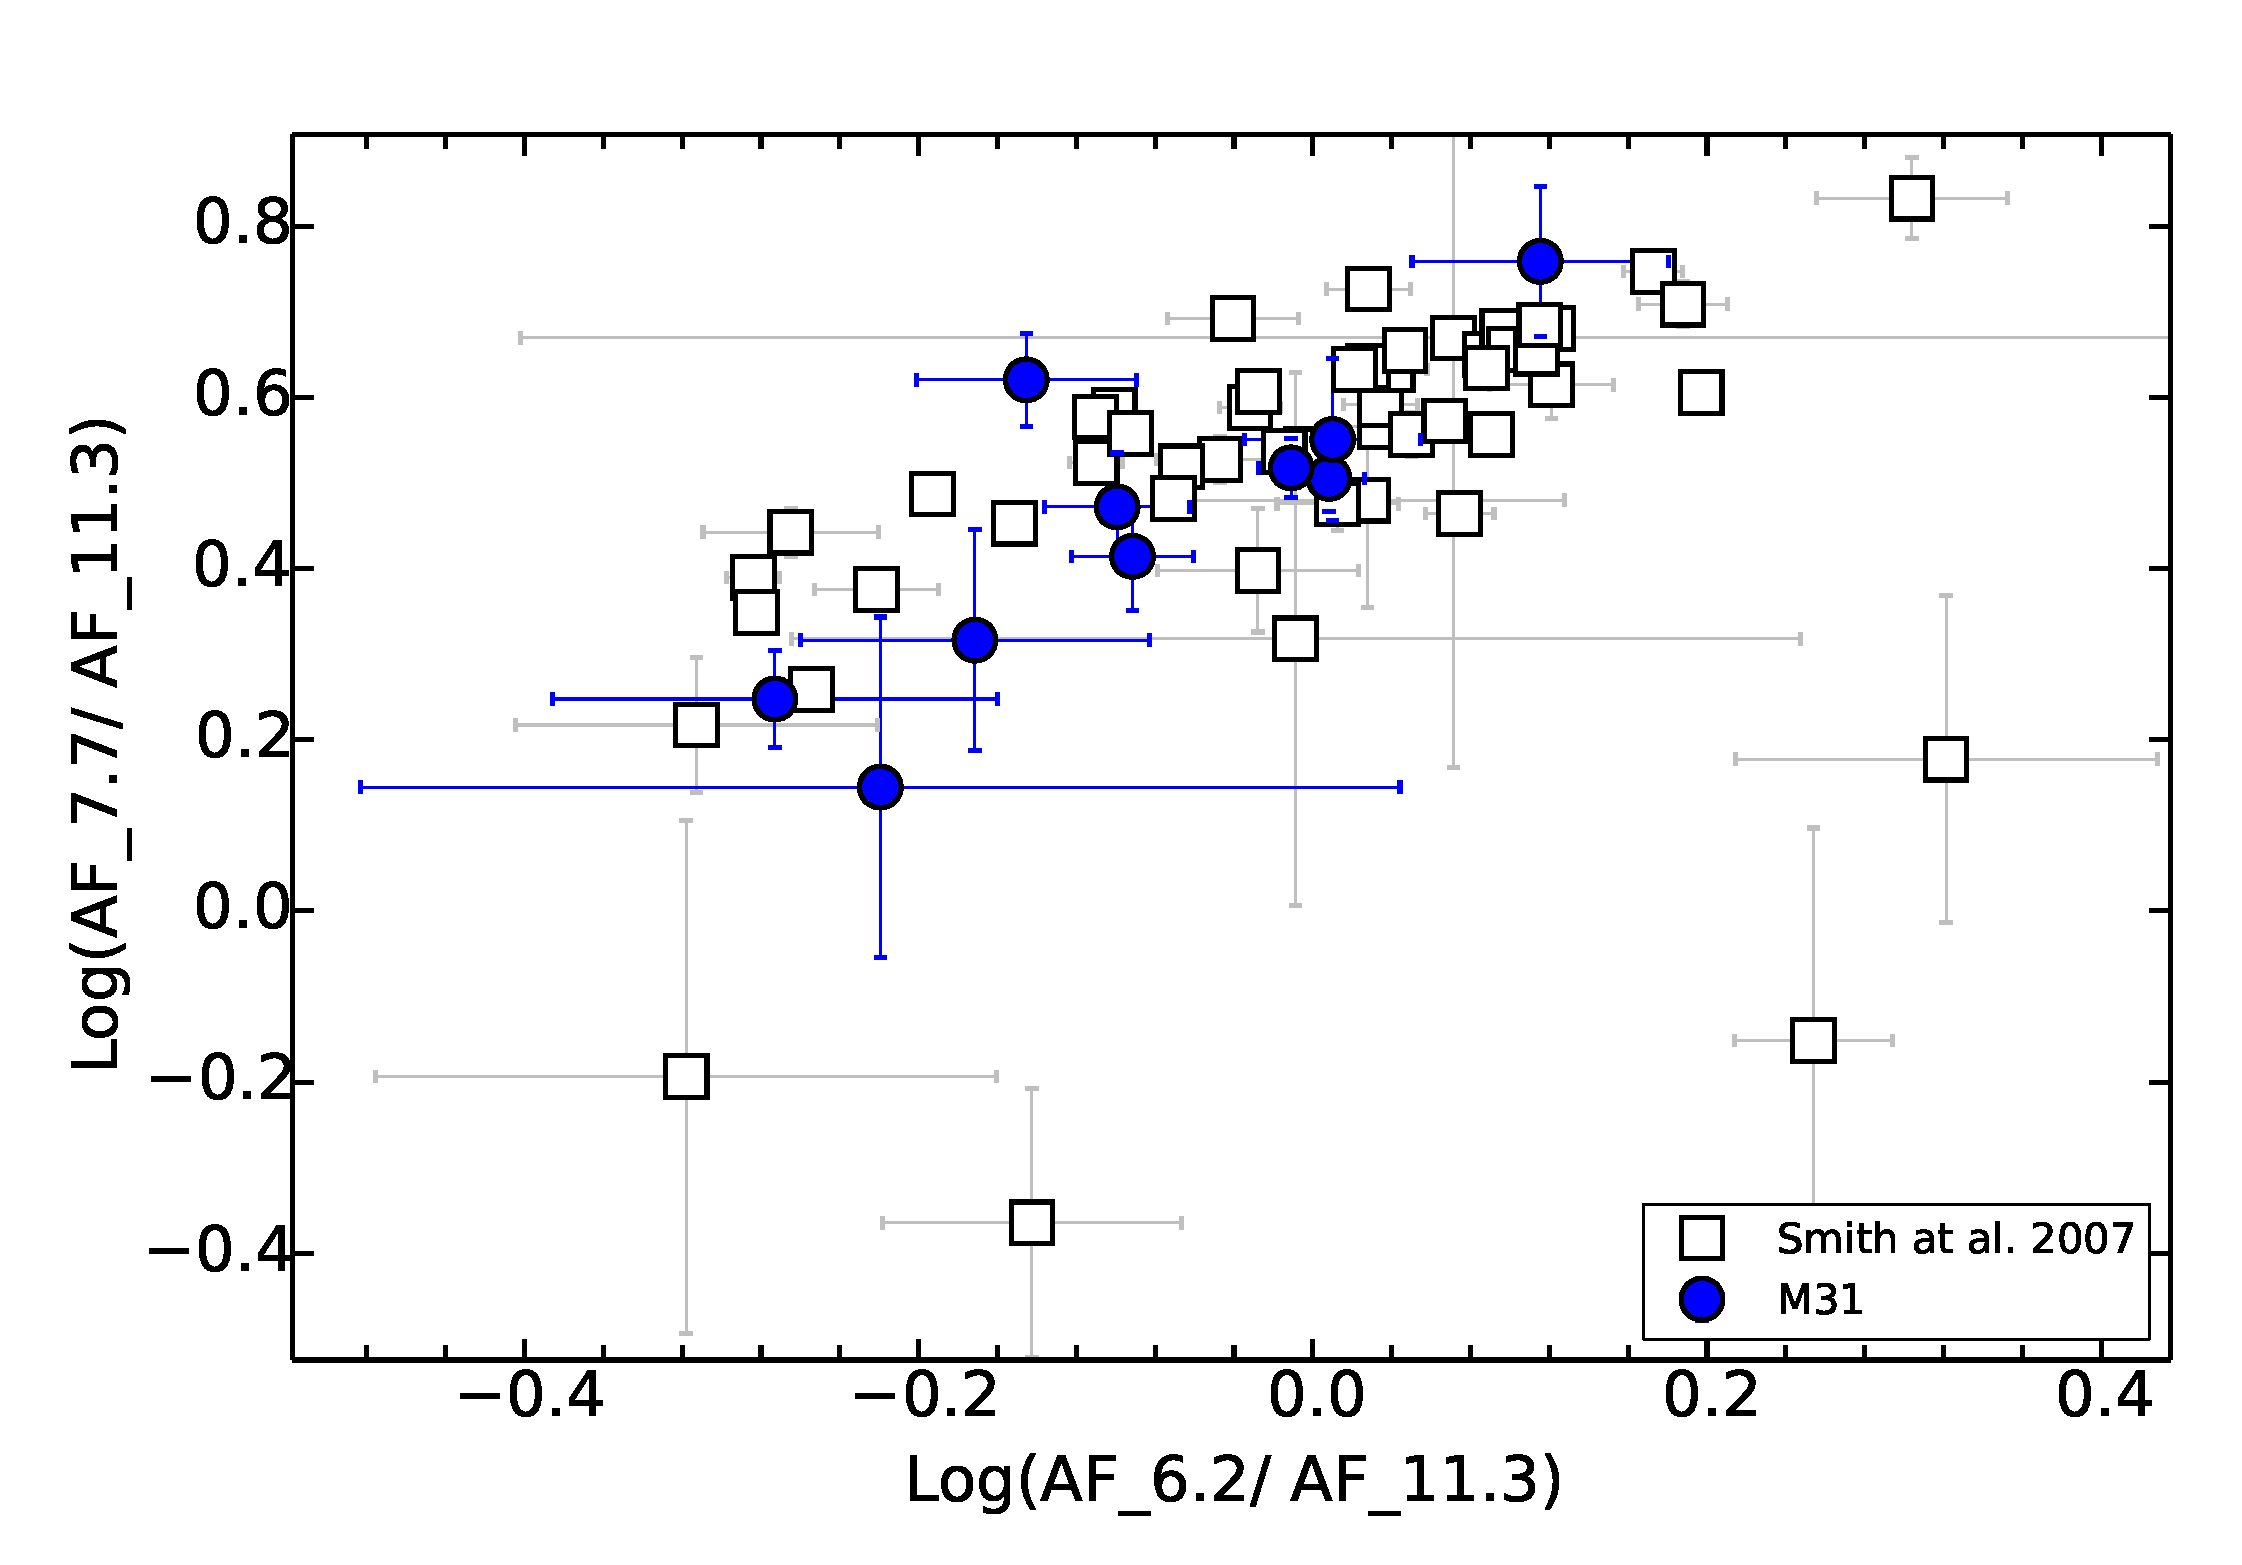
\includegraphics[scale = 0.25]{./fig9.eps}
\caption{Ratios of PAH feature fluxes (7.7~$\mu$m/11.3~$\mu$m versus 6.2~$\mu$m/11.3~$\mu$m) for 10 regions in M31.
Open squares represent the central regions of nearby galaxies as observed in the SINGS sample by \citet{Smith:2007lr}.
}
\label{PAHlines}
\end{figure}


\subsection{PAH equivalent widths versus radiation hardness and metallicity}
\label{sect:eqw_rh}

As mentioned in the introduction, PAH equivalent widths tend to decrease as radiation hardness increases,
and as metallicity decreases \citep{Calzetti:2010fk}.  
Figures~\ref{englII} and \ref{gordII} show the equivalent widths of the  8~$\mu$m feature 
(a combination of the 7.7, 8.3 and 8.6~$\mu$m PAHFIT components) and the 
 7.7 and 11.2~$\mu$m features as a function of RHI, with the starburst sample of \citet{Engelbracht_2008} 
and  H~{\sc ii} regions in M101 \citep{Gordon:2008lr} for comparison.
The M31 regions have about the same properties as the starburst galaxies and M101 H{\sc ii} regions, 
except for one M31 region with really high RHI (CHECK prob bad data) and one with really high EQW (CHECK).
No clear trend is defined by the M31 data, unsurprising given the uncertainties and the limited
number  of regions.
Figure \ref{metalicityVseqw} compares  PAH EQWs  versus  metallicity for our sample and the starburst 
galaxies of \citet{Engelbracht_2008} ( see also alternate version using Gordon data instead). 
We do not have enough data from low-metallicity regions in M31 to observe the expected decrease of PAH EQW with decreasing 
metallicity; however the M31 data occupy the same region of parameter space as the M101 data
and we conclude that the EQWs of the regions in M31 are consistent with previously published ``normal'' values.
The M31 region with very low  7.7~$\mu$m  equivalent widths is Region 8, which has
a noisy spectrum in the blue as well as substantial modelled contribution from starlight (see Figure~\ref{PAHFITplots}).


% combine following figures
\begin{figure}
\centering
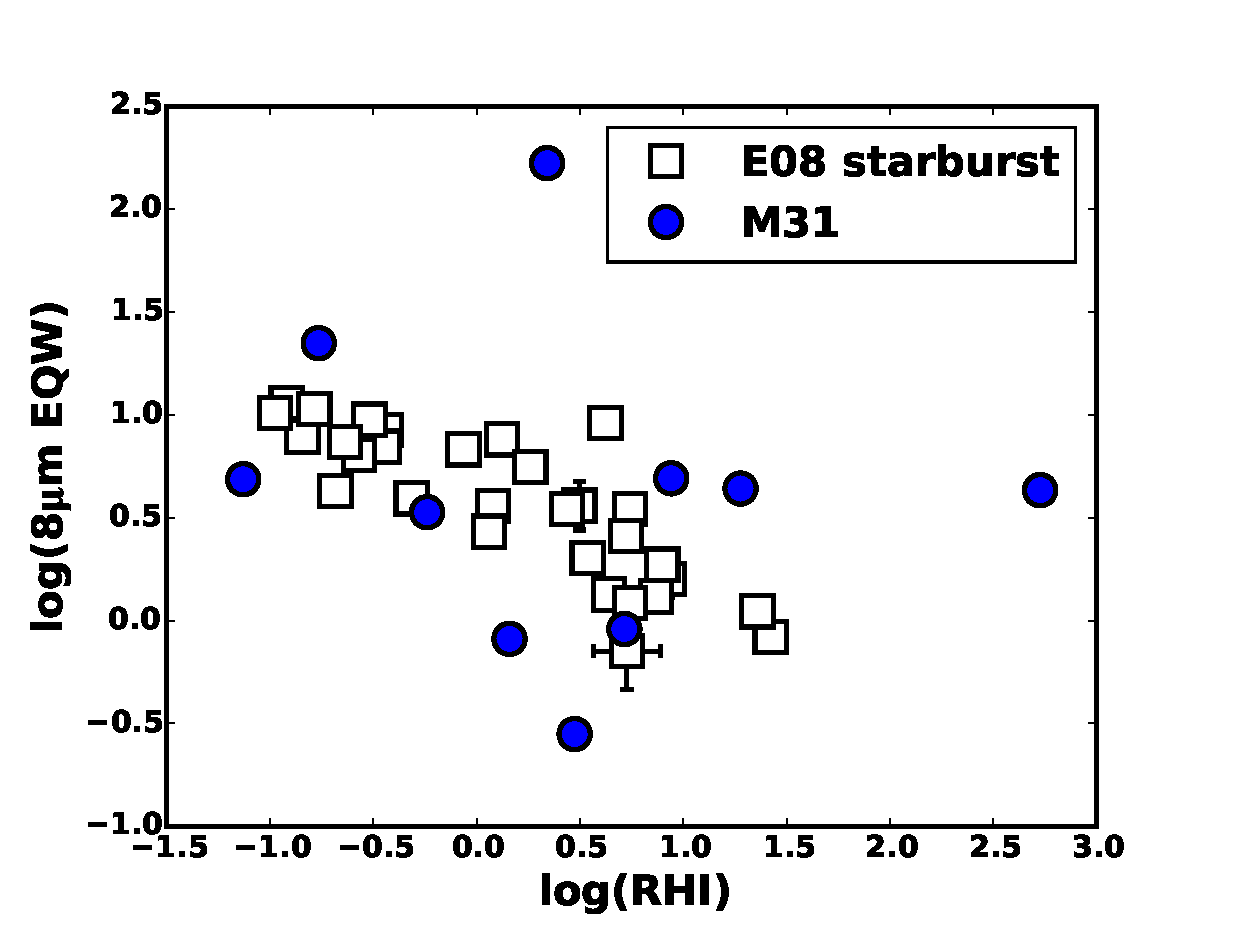
\includegraphics[scale=0.4]{./fig10_new.eps}
\caption{Equivalent width of the 8~$\mu$m PAH feature versus radiation hardness index (RHI) for the M31 sample (blue),
and the starburst galaxy sample from \citet{Engelbracht_2008} (open squares).
}
\label{englII}
\end{figure}

\begin{figure}
\centering
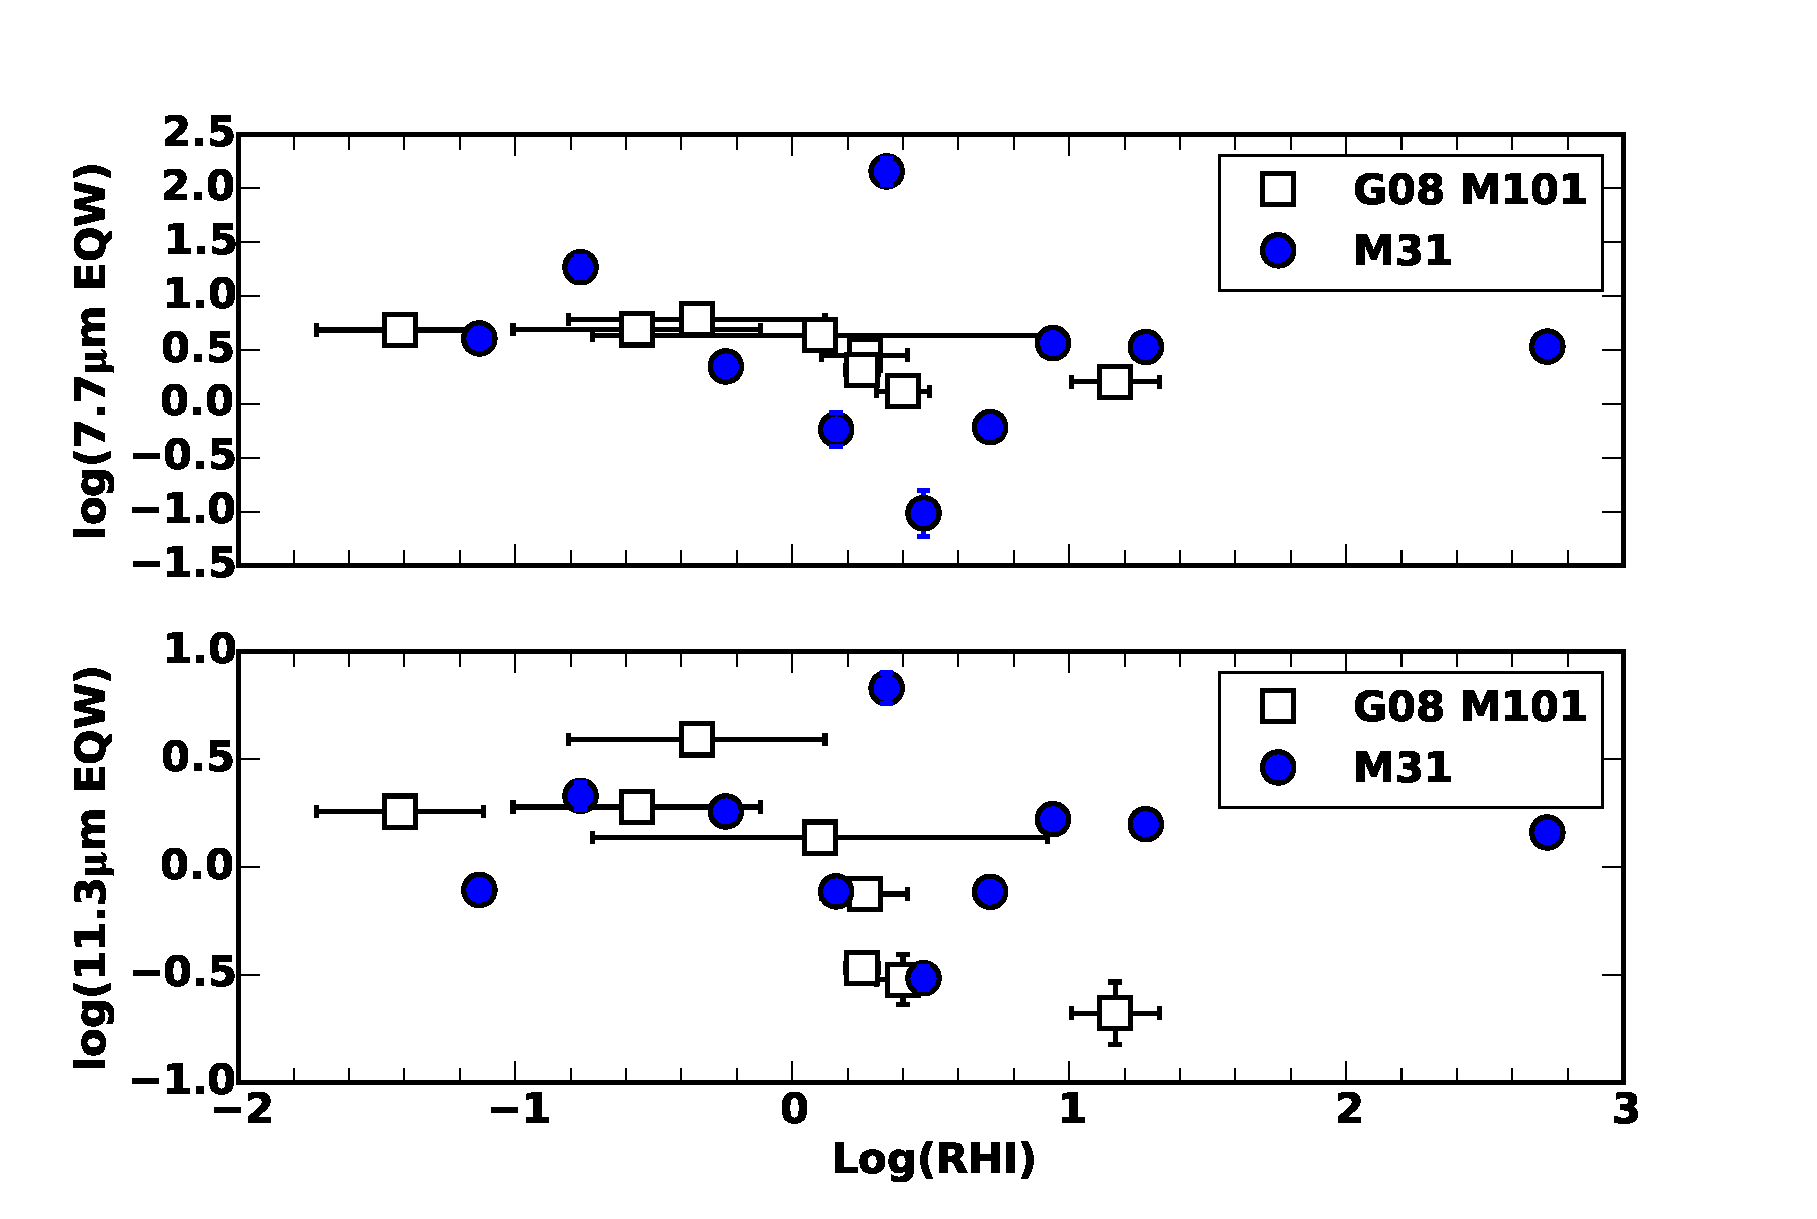
\includegraphics[scale=0.30]{./fig11_new.eps}
\caption{Equivalent widths of the 7.7~$\mu$m PAH feature (top panel) and 11.3~$\mu$m PAH feature (bottom panel) versus 
radiation hardness index (RHI) for the M31 sample. Open squares represent H~{\sc ii} regions in M101 observed  by \citet{Gordon:2008lr}.  
}
\label{gordII}
\end{figure}

\begin{figure}
\centering
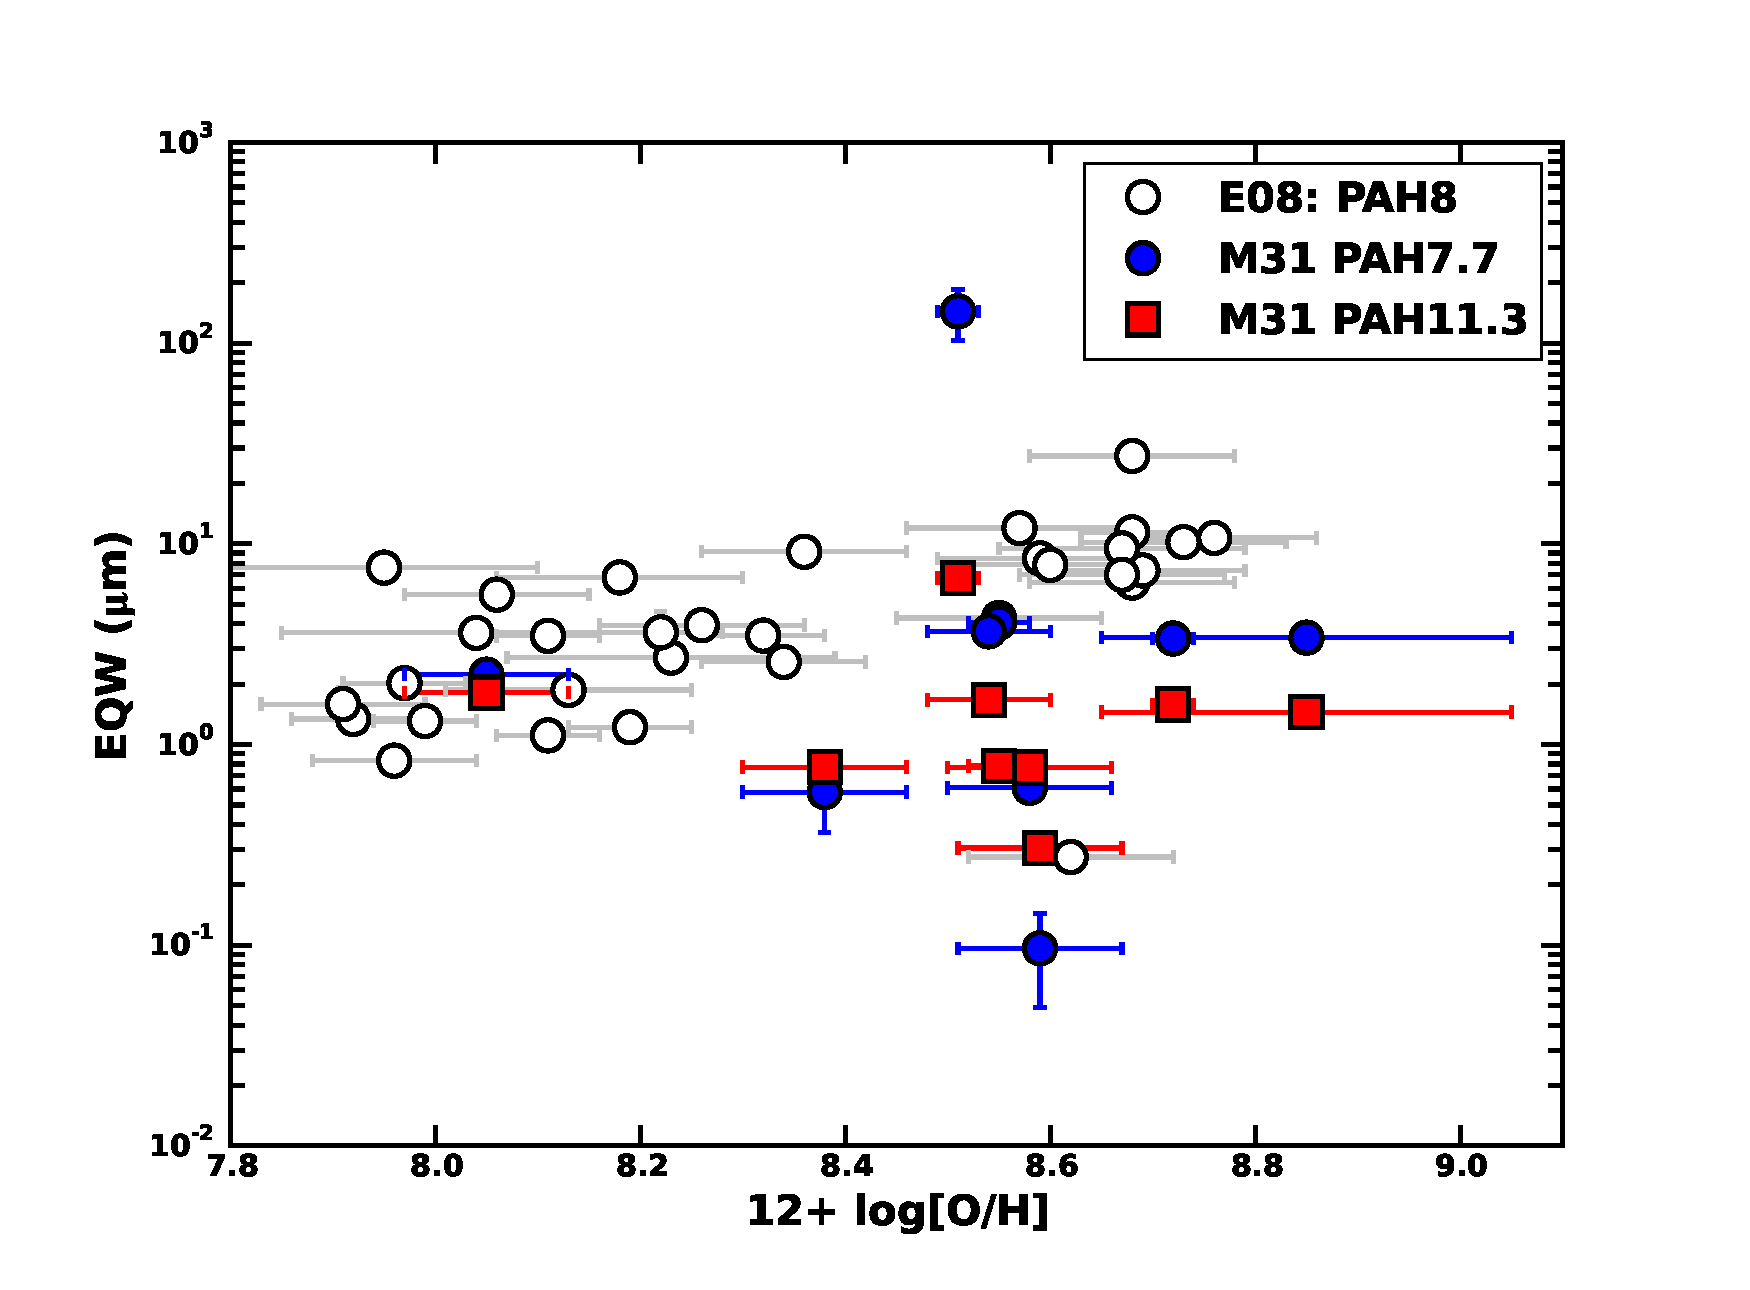
\includegraphics[scale=0.32]{./fig12_new.eps}
\caption{ PAH equivalent widths versus metallicity. 
Filled circles are M31 7.7~$\mu$m EQWs; filled squares are M31 11.3~$\mu$m EQWs; 
open circles are 8~$\mu$m EQWs for the starburst sample from \citet{Engelbracht_2008}.
Metallicities of the M31 regions have had 0.35~dex subtracted to account for the offset  between direct and strong-line measurements. 
}
\label{metalicityVseqw}
\end{figure}

\begin{figure}
\centering
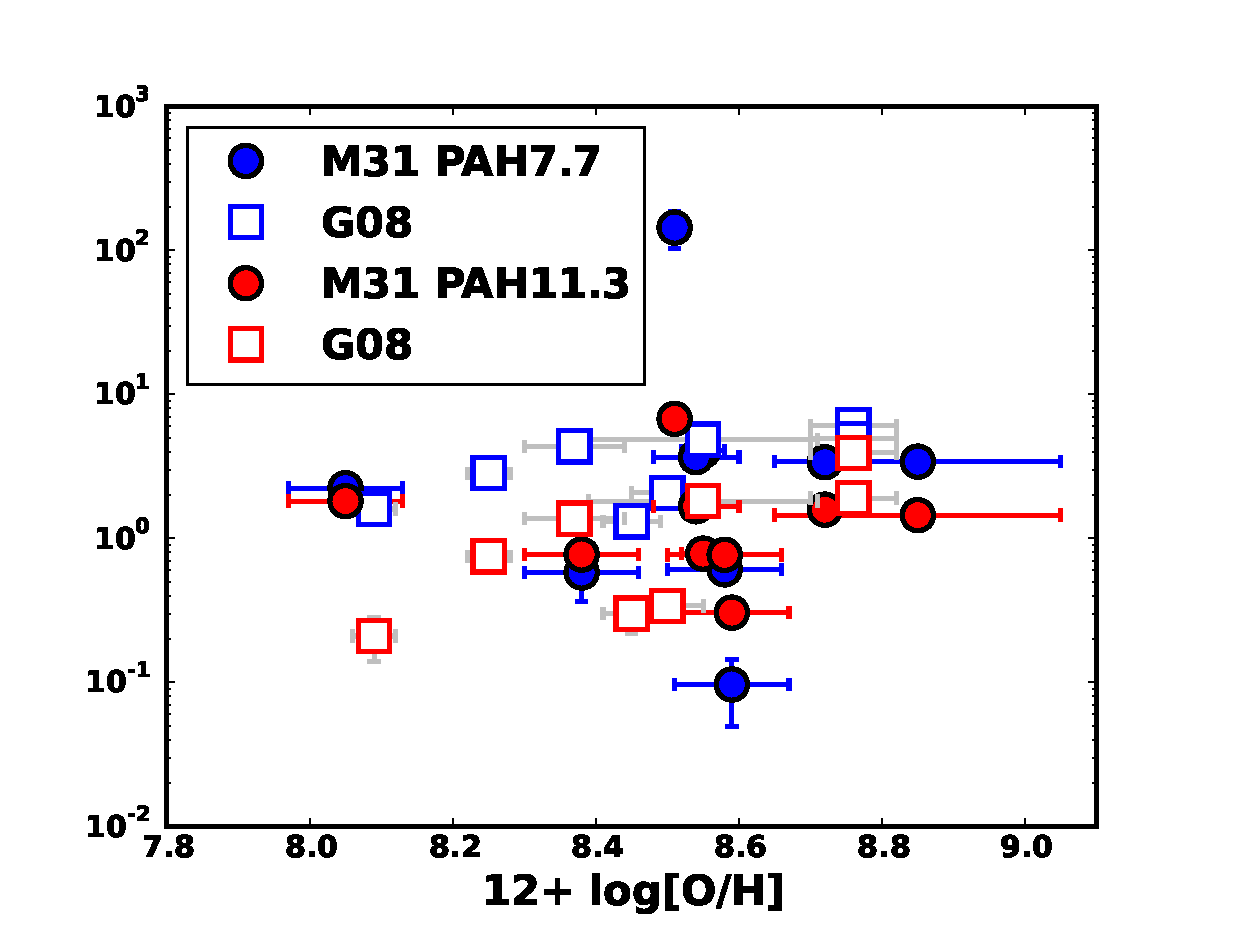
\includegraphics[scale=0.4]{./fig12a.eps}
\caption{ PAH equivalent widths versus metallicity. 
Filled circles are M31 EQWs;  open squares are M101 EQWs from \citet{Gordon:2008lr}.
Metallicities of the M31 regions have had 0.35~dex subtracted to account for the offset  between direct and strong-line measurements. 
}
\label{metalicityVseqw}
\end{figure}



